\documentclass[12pt]{article}

\usepackage[english]{babel}
\usepackage[utf8x]{inputenc}
\usepackage{amsmath}
\usepackage{graphicx}
\usepackage{longtable}
\usepackage{hyperref}
\usepackage{natbib}

\usepackage{comment}
\includecomment{todo}
%\excludecomment{changelog}
%\excludecomment{todo}

\newcommand\x         {\hbox{$\times$}}
\newcommand\othername {\hbox{$\dots$}}
\def\eq#1{\begin{equation} #1 \end{equation}}
\def\eqarray#1{\begin{eqnarray} #1 \end{eqnarray}}
\def\eqarraylet#1{\begin{mathletters}\begin{eqnarray} #1
                  \end{eqnarray}\end{mathletters}}
\def\mic              {\hbox{$\mu{\rm m}$}}
\def\about            {\hbox{$\sim$}}
\def\Mo               {\hbox{$M_{\odot}$}}
\def\Lo               {\hbox{$L_{\odot}$}}
\def\comm#1           {{\tt (COMMENT: #1)}}
\def\kms   {\hbox{km s$^{-1}$}}
\def\email#1{\href{mailto:#1}{\tt #1}}

\usepackage[usenames]{color} 
\newcommand{\G}[1]{{\color{red} #1}}
\newcommand{\B}[1]{{#1}}
\newcommand{\R}[1]{{\color{red}}}
\newcommand{\code}[1]{\texttt{#1}}



\title{Hyper Suprime-Cam Survey \\
  Pipeline Description}
\author{
  The HSC Pipeline Team: \\
  Hisanori Furusawa,
  Michitaro Koike,
  Yuki Okura, \\
  Tadafumi Takata,
  Yoshihiko Yamada (NAOJ Mitaka), \\
  Naoki Yasuda,
  Steve Bickerton,
  Sogo Mineo (IPMU), \\
  Robert Lupton,
  Jim Bosch,
  Craig Loomis, \\
  Hironao Miyatake,
  Paul Price (Princeton) \\
}


\begin{document}
\maketitle
\pagestyle{headings}

\begin{abstract}
\end{abstract}

\clearpage

\tableofcontents

\clearpage

\section{Introduction}

This document describes the Hyper Suprime-Cam Survey Pipeline, which will be used to process the survey
observations and deliver data products with a consistent high quality to the collaboration, and ultimately to
the world, for the realisation of the survey science goals.

\subsection{Hyper Suprime-Cam}

%%%
%%% Stolen from the proposal, with some edits
%%%

Hyper Suprime-Cam takes advantage of the full accessible field of view of the Subaru telescope (1.5~deg$^2$
diameter).  The focal plane is paved with 104 Hamamatsu Deep Depletion science CCDs (plus another 8 guiding
and wavefront monitoring CCDs), each 2k\x 4k. These chips, which are three-side buttable and each have four
independent readout amplifiers, are currently installed in Suprime-Cam, which has demonstrated their excellent
characteristics: low read noise, excellent charge transfer efficiency, few cosmetic defects, and most
importantly, high quantum efficiency from 4000\AA\ to 10,000\AA.  The CCD pixels are $15\mu$m on a side,
corresponding to $0.16$~arcsec at the focal plane. At this resolution, the images will be well-sampled in even
the best seeing.  Ray-tracing of the optics has shown that ghosting is minimal, with the worst ghost at an
illuminance (fractional light in a PSF aperture) of $\sim 5 \times 10^{-8}$.

Details of the instrument are summarized in the Hyper Suprime-Cam
Design Review
Booklet\footnote{\url{http://anela.mtk.nao.ac.jp/hypersuprime/presentation/hscreview20090227final_combined.pdf}}. The
official HSC
webpage\footnote{\url{http://www.naoj.org/Projects/HSC/index.html}}
provides up-to-date information.

\subsection{The HSC Survey}

%%%
%%% Stolen from the proposal, with edits
%%%

The HSC Survey was initiated to address key scientific questions using the new capabilities afforded by HSC.
The principal science drivers are:
\begin{itemize}
\item Studies of the properties of dark matter and dark energy as a
  function of redshift, using measurements of galaxy clustering, weak
  lensing, supernovae, cross-correlation with high-resolution maps
  of the Cosmic Microwave Background, and studies of high-redshift
  quasars.
\item Studies of the evolution of galaxies over cosmic time, with
  emphasis on stellar populations and star formation, morphologies, and
  active nuclei.
\end{itemize}

The survey has a classical ``wedding cake'' design, with three layers.  The Wide layer will cover roughly
1,400~deg$^2$ in five broad filters ($grizy$), with exposure times of $10-20$~min per pointing (and one with a
shorter exposure time of $\sim 30$~sec to enable astrometric and photometric calibration with other surveys).
This will go to a point-source depth of $r\sim 26$, and is optimized for weak-lensing science.  Using galaxies
for weak lensing will require exquisite understanding of their properties and evolution, which will be the
motivation of the Deep layer, covering 27~deg$^2$ in four distinct fields, going roughly one magnitude deeper
with exposures of roughly 1~hr per filter.  In addition to the broad-band filters, the Deep layer will include
imaging in three narrow-band filters, to detect Lyman-$\alpha$ emitters and study their luminosity function
and clustering properties at $z = 2.2$, 5.7, and 6.6.

To study the faintest and most distant galaxies, and to probe the
transient universe, especially high-redshift supernovae, will require
the Ultradeep layer, going another magnitude fainter yet.  Narrow-band
filters in the Ultradeep layer will search for Lyman-$\alpha$
emitters at $z = 5.7$, 6.6, and 7.3 at the very faint end of the
luminosity function.

\subsection{This document}

This document provides a reference to the HSC Pipeline which will be
used to process the HSC Survey observations, producing the necessary
data to achieve the scientific goals of the survey.  It is
especially intended for HSC Survey scientists to evaluate the pipeline
and its products in relation to their own science goals.

In section \ref{sec:pipeline}, we outline the pipeline construction and operations, tracing the flow of data
through the various stages of the pipeline, to the ultimate releases to the collaboration.  Next, in section
\ref{sec:products}, we outline the various products that will compose the data releases, with particular
attention to the measurements that comprise the catalog in the database.  Section \ref{sec:algorithms} gives
details as to the algorithms used to make these measurements, and section \ref{sec:interfaces} describes how
the data will be made available.  Finally, section \ref{sec:support} contains pointers on resources available
for supporting users of these data.


\section{The HSC Pipeline}
\label{sec:pipeline}
\subsection{Software}

%%%
%%% Stolen from the proposal
%%%

To construct the HSC pipeline, we use the LSST pipeline software as the foundation.  This is a synergistic
effort, since the pipelines have similar functionality.  By this scheme, the HSC pipeline has features and a
maturity it would not otherwise have at this stage, and because our pipeline is based on code with a larger
market share than ours could ever have alone, we can have greater confidence in the results.  In return, LSST
gains testing and verification with real-world data.  However, since LSST is a larger-scale development
project not entirely within our control, we are selective about the LSST components we use for the HSC
pipeline, so that we are not chained to every design decision of LSST.  We have also supplemented LSST
components with different algorithms, and added new pipeline components as necessary.  The LSST code is
released under the GNU Public License, version 3 (or later), and our releases of our modified versions of that
code, and our own code (as a ``derivative work'') are bound to use the same license.

The pipeline is written in Python, using C++ for low-level algorithmic components where speed is important.
SWIG is used to wrap the C++ components so they can be called directly from Python.  The combination of these
results in all the ease and flexibility of a scripting language while retaining the power of a compiled
language.

Particular attention has been paid, in large part because of our contributions, to making the LSST pipeline
extensible and configurable.  New camera interfaces and new measurement algorithms can be added without the
need to redesign or even rebuild the software.  The modular design also allows for algorithms to be
substituted at run-time, so that the pipeline can adapt to the data being processed.  These features, besides
being useful for our adaptation of the LSST pipeline to HSC, mean that we could use our own pipeline to
process data from other telescopes and cameras for comparison with the results of other pipelines (e.g., we
can not only compare the results of the HSC Survey + HSC pipeline with DECam + DES pipeline, but also with
DECam + HSC pipeline, for better diagnosis of any problems).  Interface packages have been written for LSST
simulated images (``ImSim''), CFHT MegaCam, Subaru's Suprime-Cam, SDSS, the Space Surveillance Telescope
(SST), DECam, and HSC simulated images.

Testing with archival Suprime-Cam data (in particular, from after August 2008 when the Hamamatsu CCDs were
installed) and more recently with HSC commissioning data has been an integral part of the pipeline development.

\subsection{Data flow}

The pipeline consists of multiple stages in order to produce the variety of data products required to meet the
various survey science goals.  The stages share a great deal of framework code, but differ by their inputs,
parallelism scheme (CCD vs exposure vs sky patch) and outputs.  Different science applications will depend on
different pipeline stages, according to the desired measurements, depth and accuracy.

\begin{figure}[!htbp]
    \centering
    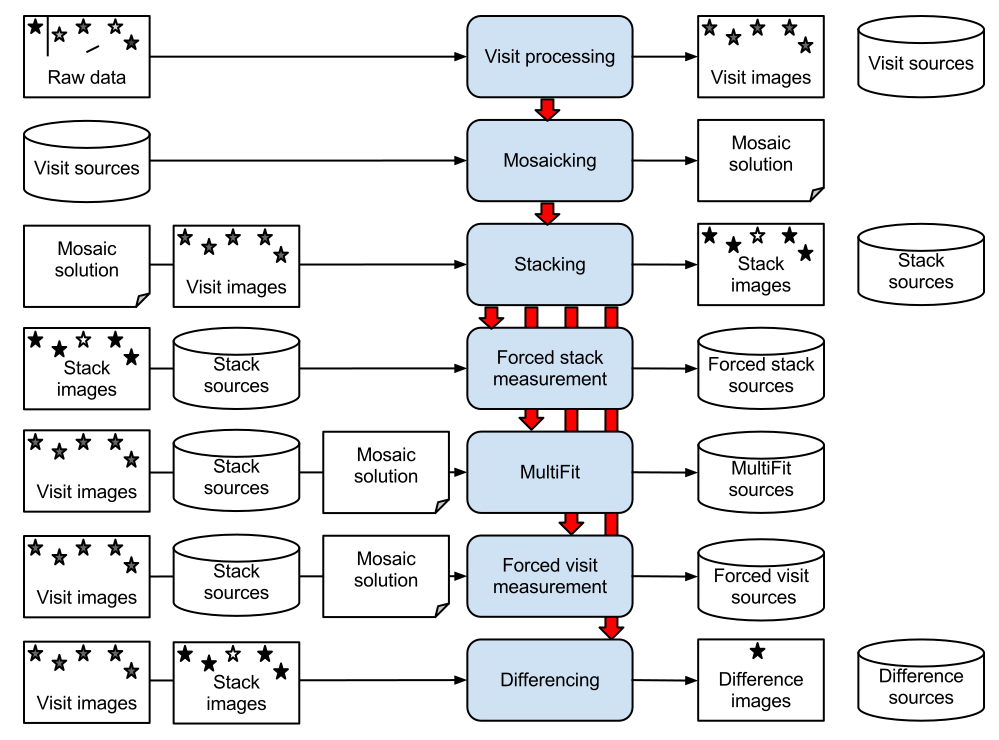
\includegraphics[scale=0.5]{figures/HSCpipelinesketch}
    \caption{HSC Pipeline data flow\label{fig:flow}}
\end{figure}

Figure~\ref{fig:flow} shows a schematic representation of the HSC pipeline.  Input data on the left is fed
into the pipeline stages (light blue, center) to produce the outputs on the right.  The first three stages
(visit processing, mosaic solution, stacking) are executed in sequence, after which all the remaining stages
can be run in parallel.  The stages are explained in more detail below.

\subsubsection{Visit processing}

Visit processing removes the instrumental signature (overscan, bias, dark, flat, bad pixels, amplifier
crosstalk) from each CCD and flags suspected cosmic-rays.  The result is a clean image for which the intensity
is a linear function of astrophysical flux\footnote{Excepting flat-field inaccuracies, and intrinsic pixel
  shape non-linearities.}  The background is estimated and removed, then bright sources on the image are used
to measure the PSF and the astrometric solution and photometric zero-point, before a final detection and
measurement pass.  From the individual CCD measurements, we determine and apply an exposure-wide astrometric
solution and photometric zero-point.

The ouputs are:
\begin{itemize}
\item Image
\item PSF
\item Background
\item Sources
\item Astrometric solution
\item Photometric zero point
\end{itemize}

\subsubsection{Mosaic solution}

Once several exposures overlapping the same part of sky are available, we can determine a mosaic solution.
This involves solving for consistent astrometric solutions and photometric zero-points for the set of
exposures, using sources in common to multiple exposures, in the same manner as \citet{2008ApJ...674.1217P}.
This allows increased accuracy and precision relative to the visit processing, by allowing use of stars
fainter than in our original reference catalog (e.g., SDSS), and incorporating spatial information unavailable
from single exposures.


\subsubsection{Stacking}

Stacking involves the coaddition of multiple images to produce a single, deeper image.  We apply the results
of mosaic solution to the input images, warp them to a common coordinate system (``sky map'';
\S\ref{alg:skymap}) and stack the pixels.  Then we will detect and measure sources on the stack.  Our code
includes a couple of recent innovations to increase the quality of the stacks.

Stacks are normally produced by first subtracting the background, but determining the background from
individual visits separately is problematic (because different choices can be made in each), commonly observed
as dark rings around bright stars and galaxies.  Instead, we perform ``background matching''
(\S\ref{alg:backgroundMatching}) to produce a stack with a high signal-to-noise realisation of the background
in a single reference exposure.  This background can then be measured over wide scales and subtracted with a
high degree of accuracy.

It must always be remembered that a stack is a computational convenience, rather than a perfectly accurate
representation of the sky.  Indeed, if the seeing is not constant with time it becomes impossible to produce a
stack with a PSF varying in a continuous fashion over the field, unless we deliberately degrade the data by
convolving the inputs to a common PSF.  In order to attempt to deal with the discontinuous PSF, we use a
``CoaddPsf'' (\S\ref{alg:coaddPsf}), which is a sum of the PSFs of the input images at each point of interest.

Unfortunately, degrading the PSF is the only way of accurately measuring the colors of galaxies (e.g., for
photometric redshifts) from stacks in the presence of color gradients and seeing changes.  For this reason, we
will produce ``PSF-matched stacks'' for the purpose of measuring galaxy colors.  But because these data have
been deliberately degraded, they are not the deepest available, so we will also produce ``deep stacks'' by
coadding without PSF matching.

Despite the intrinsic limitations of stacks, the measurements from this pipeline stage will be useful for
applications where extreme accuracy isn't required, e.g., searching for sources with extreme spectral features
such as high-$z$ quasars.  The deep stacks will also be used to identify discrete astrophysical objects for
the following stages that require known object positions.

\subsubsection{Forced Stack Measurement}

The deep stack catalog of a nominated band ($i$-band) will be used as a reference to measure sources in
PSF-matched stacks, with the same centroids and apertures.  This provides matched-aperture galaxy colors,
e.g., for photometric redshifts.  Because of the limitations of the stacks, these are not the most accurate
measurements available, but they are more simple and will be available earlier than the full MultiFit
measurements.

\subsubsection{MultiFit}

%%%
%%% Stolen from LSST Data Products document, edited
%%%

The deep stack catalog of a nominated band ($i$-band) will be used as a reference to measure the sources in
multiple bands.  However, rather than coadding a set of images and measuring object characteristics on the
coadd, MultiFit fits a PSF-convolved model simultaneously to multiple independent observations of an
object. This reduces systematic errors, improves the overall signal-to-noise, and allows for fitting of
time-dependent quantities degenerate with shape on the coadds (for example, the proper motion). The models we
plan to fit will not allow for flux variability.  We expect these will be the best possible measurements of
the position, shape and flux of objects of constant flux.

\subsubsection{Forced Visit Measurement}

The deep stack catalog of a nominated band ($i$-band) will be used as a reference to measure the sources in
every available visit.  This produces time-resolved positions (for proper motions and parallax) and fluxes
(for light curves).


\subsubsection{Differencing}

The deep stack images will be used as references to be subtracted from individual visits (or
nightly/monthly/yearly stacks of visits) in order to identify and measure transients.  We will use PSF matching
(\S\ref{alg:psfMatching}) to minimise false positives, but further work will be needed to produce a clean
candidate list.

At the present time, the differencing stage has been greatly neglected in the development of the pipeline, as
more fundamental operations have received priority.  We have prototype code for PSF matching that needs to be
cleaned up, made more robust, and thoroughly tested.  Nevertheless, we are committed to delivering the
differencing stage in advance of the second year of operations for the supernova/transient campaign.


\subsection{Releases}

Data releases are the culmination of the pipeline development and operations, whereby the results are delivered
to the collaboration for science use.

\subsubsection{Daily}

When particular observations have been declared by the transients working group as useful for the
identification of transients (SNe, GRBs), we will attempt to process those observations promptly through a
limited set of the pipeline stages --- visit processing, forced CCD measurements and differencing --- and
deliver the results to the transients working group by 4pm Hawaiian Standard Time the following day.  {\bf It
  should be understood that these releases will be preliminary, and made on a best-efforts basis.}  The
released data will be in the form of FITS images and FITS tables, using the pipeline's internal formats, and
will be placed in a suitable location for bulk download by the transients working group members.

\subsubsection{Monthly}

Aware of the great interest in the HSC survey observations by the collaboration members, and desiring to
encourage independent quality analyses, we will endeavour to produce a preview of the processed data (through
all the pipeline stages) to the collaboration as soon as possible after the observing run.  {\bf It should
be understood that these releases will be preliminary, and made on a best-efforts basis.}  The released data
will be in the form of FITS images for bulk download and a database accessed in the usual manner.

Once the survey is sufficiently progressed that a single month's data is not as interesting, we may not post
the preview, though reducing the data promptly is necessary to inform the observing plan for the following run
of unsuitable exposures in the previous run.


\subsubsection{Semi-annually}

The semi-annual releases are the main goal of the pipeline team.  As part of each, it is our intention to
re-reduce all data from the survey with the best available code and calibrations, delivering all the data
products (\S\ref{sec:products}) to the survey collaboration.  Each semi-annual release will be formally
announced on the HSC mailing list\footnote{\email{hsc@astro.princeton.edu}}, and accompanied by a set of
release notes identifying features and known bugs\footnote{We guarantee that no release will be free of bugs.}
in the release.  The released data may be accessed through the methods described in \S\ref{sec:interfaces}.


\section{Data Products}
\label{sec:products}

Here we describe the various data products produced by the pipeline.

\subsection{Images}

Images from the pipeline shall be multi-extension FITS (MEF) files, containing the image data, mask plane and
variance plane.  The World Coordinate System (WCS) in the headers shall use the \code{TAN-SIP} convention
\footnote{\url{http://fits.gsfc.nasa.gov/registry/sip.html}}, except for those corresponding to a tract/patch
(\S\ref{alg:skymap}) which shall use the standard \code{TAN} projection.  The FITS files may also Contain
further extensions (e.g., for the PSF).  We encourage the use of our software in reading and manipulating the
files.

The images are provided principally for the sake of verifying candidates, quality analysis, and to enable
extensive analyses not supported by the pipeline.  If you desire the images in order to generate your own
catalogs (e.g, with SExtractor), please consider using the pipeline catalogs instead, as this will benefit
everybody (e.g., you will have frequent updates with the latest code, and any problems you find can be fed
back into the pipeline).  If the particular measurement you desire to have is not available, please let us
know so that we attempt to support it.

\subsubsection{Visits}

The visit images shall be a single MEF for each CCD, which is background-subtracted and possesses a common
astrometric solution and photometric zero point with the entire visit.  The MEFs shall also include PSF models
for each.  The background model is saved separately, and available if desired.

\subsubsection{Stacks}

The stack images shall be a single MEF for each patch, with a pre-defined astrometric solution and photometric
zero point.  The MEFs shall also include a CoaddPsf (\S\ref{alg:coaddPsf}) for each.

\subsubsection{Differences}

The difference images shall be a single MEF for each patch, with a pre-defined astrometric solution for each,
and a photometric zero point calculated from the original visit.  The MEFs shall also include a suitable PSF
model for each.

\subsection{Catalogs}

The catalogs are the principal data product produced by the pipeline.  It is our goal that most of the science
projects of the survey collaboration can be performed almost entirely from the catalogs; this was the
experience for SDSS.  We encourage collaboration members to discuss with us the addition of particular
measurements or flags that are lacking in the catalogs, so that we can develop and include them.

Catalogs are stored internal to the pipeline as FITS tables.  In these tables, the flags are combined into
a single bit array (FITS format code \code{X}); your software may or may not recognise the flag names in the
header.  In general, it should not be necessary for those outside the pipeline team to read these FITS tables,
as the database (\S\ref{sec:database}) should contain all the same information.

\subsubsection{Visits}

The following measurements will be made as part of the visit processing:
\begin{itemize}
\item Centroid, with error estimate.
\item Flux from PSF photometry, with error estimate.
\item Flux from aperture photometry, with error estimate.
\item Kron flux, with error estimate.
\item Petrosian flux, with error estimate.
\item Gaussian model flux, with error estimate.
\item Adaptive moments.
\item Star/galaxy indicator.
\end{itemize}

\subsubsection{Stacks}

Because we use a CoaddPsf (\S\ref{alg:coaddPsf}), the flags regarding the PSF will not be populated, though
they may be defined.

The following measurements will be made as part of the stack processing:
\begin{itemize}
\item Centroid, with error estimate.
\item Flux from PSF photometry, with error estimate.
\item Flux from aperture photometry, with error estimate.
\item Kron flux, with error estimate.
\item Petrosian flux, with error estimate.
\item Gaussian model flux, with error estimate.
\item Adaptive moments.
\item Shapes from the regaussianization method.
\item Flux from MultiShapelet algorithm, with error estimate.
\item Star/galaxy indicator.
\end{itemize}

\subsubsection{Forced Visit Measurements}

The following measurements will be made as part of the forced visit measurements:
\begin{itemize}
\item Centroid, with error estimate.
\item Flux from PSF photometry, with error estimate.
\item Flux from aperture photometry, with error estimate.
\item Kron flux with reference aperture, with error estimate.
\item Petrosian flux with reference aperture, with error estimate.
\item Gaussian model flux with reference aperture, with error estimate.
\item Star/galaxy indicator.
\end{itemize}

\subsubsection{Forced Stack Measurements}

The following measurements will be made as part of the forced stack measurements:
\begin{itemize}
\item Centroid, with error estimate.
\item Flux from PSF photometry, with error estimate.
\item Flux from aperture photometry, with error estimate.
\item Kron flux with reference aperture, with error estimate.
\item Petrosian flux with reference aperture, with error estimate.
\item Gaussian model flux with reference aperture, with error estimate.
\item Flux from MultiShapelet algorithm with reference aperture, with error estimate.
\item Star/galaxy indicator.
\end{itemize}

\subsubsection{MultiFit}

The following measurements will be made as part of MultiFit:
\begin{itemize}
\item Centroid, with error estimate.
\item Flux from PSF photometry, with error estimate.
\item Flux from aperture photometry, with error estimate.
\item Kron flux, with error estimate.
\item Petrosian flux, with error estimate.
\item Gaussian model, with error estimate.
\item Flux from MultiShapelet algorithm, with error estimate.
\item Star/galaxy indicator.
\end{itemize}


\subsubsection{Differences}

The following measurements will be made as part of differences processing:
\begin{itemize}
\item Centroid, with error estimate.
\item Flux from PSF photometry, with error estimate.
\item Flux from aperture photometry, with error estimate.
\item Kron flux, with error estimate.
\item Petrosian flux, with error estimate.
\item Gaussian model, with error estimate.
\item Star/galaxy indicator.
\end{itemize}


\subsection{Database}
\label{sec:database}
\subsubsection{Schema}

\section{Algorithms}
\label{sec:algorithms}

Here we describe the various algorithms used within the pipeline.  Of particular interest are the flags
(\S\ref{alg:flags}) and measurements (\S\ref{alg:measurements}) that will comprise the source catalogs
produced in each pipeline stage, and ingested into the database.  Then follows various general algorithms
used in the pipeline.

\subsection{Flags}
\label{alg:flags}

Flags are binary decisions made about each object, and are useful for indicating how a measurement of that
object should be interpreted, and if it is trustworthy.

\subsubsection{Pixel flags}

Pixel flags are flags set on the basis of pixel characteristics.  They comprise:
\begin{itemize}
\item \code{flags.pixel.edge} is set if the source is near the edge of the frame (where the signal-to-noise
  requirement for detection is higher due to the convolution involved; and where measurements may be subject to
  failure).
\item \code{flags.pixel.bad} is set if any pixels in the source footprint have been masked as \code{BAD}
  (typically non-functioning detectors, or severely vignetted areas).
\end{itemize}

The following flags indicate whether the source has been affected by a variety of conditions.  There are two
modes for each: \code{<flag>.any} is set if any pixels in the source footprint have been affected (and
therefore measurements may be impacted only subtly), while \code{<flag>.center} is set if any pixels in the
$3\times 3$ region about the peak have been affected (and therefore measurements may be drastically wrong).

\begin{itemize}
\item \code{flags.pixel.interpolated}: pixels masked as \code{INTERP}, i.e., have been interpolated over, and
  are therefore not the original pixels; this is done for saturated pixels and cosmic rays.
\item \code{flags.pixel.saturated}: pixels masked as \code{SAT}, i.e., are saturated (over full well depth).
\item \code{flags.pixel.suspect}: pixels masked as \code{SUSPECT}, i.e., are non-linear.
\item \code{flags.pixel.cr}: pixels masked as \code{CR}, i.e., suspected cosmic-ray.
\end{itemize}

\subsubsection{Algorithm flags}

Each measurement algorithm (\S\ref{alg:measurements}) has a corresponding algorithm flag that, if set,
indicates the measurement failed; typically this means an exceptional conditional was encountered, such as the
source being too close to the edge.  These algorithm flags are named after the measurement with \code{.flags}
appended, e.g., \code{flux.gaussian.flags}.

Many flux measurement algorithms have an additional flag that may be set if performing the flux measurement on
the PSF at the position of the object failed, and therefore the PSF flux correction cannot be applied (see
\S\ref{alg:measurements}).  These are named after the measurement with \code{.flags.psffactor} appended.

\subsubsection{Calibration flags}

\begin{itemize}
\item \code{calib.detected} is set if the source was detected in calibration (as a bright source).
\item \code{calib.psf.candidate} is set if the source was selected as a candidate PSF star.
\item \code{calib.psf.used} is set if the source was actually used in determining the PSF.
\end{itemize}

\subsubsection{Deblending flags}

The deblender (\S\ref{alg:deblender}) sets some flags based on its interpretation of the source:
\begin{itemize}
\item \code{deblend.deblended-as-psf} is set if the deblender considered the source as a PSF.
\item \code{deblend.too-many-peaks} is set if the deblender attempted to divide the source beyond a limit;
  only the brightest peaks were deblended.
\item \code{deblend.failed} is set if deblending failed on this source.
\end{itemize}

\subsubsection{Other}

\begin{itemize}
\item \code{flags.negative} is set if the source was detected as a negative (principally used in the
  difference stage).
\item \code{flags.badcentroid} is set if the principal centroid algorithm (used to feed all other algorithms)
  failed.
\end{itemize}

\subsection{Measurements}
\label{alg:measurements}
\subsection{Background Matching}
\label{alg:backgroundMatching}

We use the algorithm of \citealt{2011arXiv1111.6958H}, extended to two-dimensional data, which avoids the
common problem of increased noise from over-subtracting the background; this technique will be important for
reaching the maximum depth in the Deep and Ultradeep fields.

\subsection{PSF}
\subsection{CoaddPsf}
\label{alg:coaddPsf}

Measurements on the stacks will use a PSF constructed from those of the input images (known as ``StackFit'',
pioneered by \citealt{2012arXiv1210.2732J} on the Deep Lens Survey).  In this way, we can accurately follow
the complicated (and discontinuously variable) PSF over the stacked image.  We expect these measurements will
be scientifically useful in their own right, and they will be available relatively quickly, but will not be
the most accurate possible because the stacking process necessarily discards data.

\subsection{Skymap}
\label{alg:skymap}

The ``skymap'' is a tessellation of the sky, providing suitable pre-defined coordinate systems for operations
on the sky such as stacking.  The sky map divides the sky into ``tracts''.  For convenience and parallelism,
each tract is sub-divided into ``patches''.  Tracts and patches overlap, so that sources are not lost in the
gaps.  These overlaps can be both annoying (additional care is required to remove duplicate sources) and
useful (additional source of quality checking).

Our tracts tangent planes (\code{TAN} WCS) distributed in rings of Declination, which matches well with the
survey geometry.  This has more inefficiency (tract overlap) at the pole, but since our survey doesn't cover
that area, it's not a problem.  Individual tracts are roughly the same size as the field of view of HSC, and
have North and East vectors aligned with the columns and rows, respectively.

\begin{figure}[!htbp]
    \centering
    \includegraphics[scale=0.3]{figures/rings_equat.png}
    \includegraphics[scale=0.3]{figures/rings_pole.png}
    \caption{Demonstration of the skymap scheme we will use for the HSC pipeline.  Left: Equatorial
      projection.  Right: Polar projection.  Note that the tracts shown here are very much larger than we will
      use in practise; the large tracts allows the characteristics of the tessellation (e.g., the larger
      overlap at the poles) to be more clearly discerned.\label{fig:skymap}}
\end{figure}

\subsection{Mosaic}

For each exposure we can calibrate both astrometry and photometry using measurements of objects
matched with reference catalog. But the number of objects are limited by reference catalog and
the we may be affected by some systematic effects. Using multiple exposures and simultaneous fitting
on them enable us more reliable and systematics free calibration. This is known as "uber-calibration" and
applied to SDSS and Pan-STARRS1 photometry. In the pipeline we apply the same kind of method
to each tract. "Uber-calibration" for entire survey region is a separate problem and not yet implemented.

In our meas\_mosaic package we use both catalog matched objects and non-matched objects.
Non-matched objects will be spatially matched between exposures based on astrometry determined 
by chip based analysis. Requirements for non-matched objects having consistent positions/fluxes
contribute to better relative (internal) consistency and requirements for catalog matched objects 
contribute to absolute (external) consistency. 

In astrometry optical distortion of the system is modeled by polynomial functions of focal plane coordinates.
We determine the coefficients of polynomials for each exposure. The locations of CCDs on the focal plane
(offsets and rotations) are also fitting parameters.
In photometry correction for the flat-field is modeled by polynomial functions of focal plane coordinates.
Same as astrometry, the coefficients of polynomials are determined. Relative flux scales between exposures
are also determined.

The mathematical functional forms are the following.

In the following, super(sub)scription $s$, $e$, and $c$ denotes stars, exposures and chips, respectively.
$(x,y)$ is a pixel coordinate within a chip, $(u,v)$ is a focal plane coordinate, $(\xi,\eta)$ is an projected
celestial coordinate of the sky at $(A,D)$.

For astrometry, we solve the equation for $\Delta a_k^e$, $\Delta b_k^e$, $\Delta X_c$, $\Delta Y_c$, and
$\Delta\theta_c$ until it converges. For non-matched sources $\Delta\alpha^s$ and $\Delta\delta^s$ are also
solved.  For matched sources their catalog values are used for their $(\alpha, \delta)$ and they are fixed.
$\chi^2$ equation is linearized at eq (5). Initial values are estimated from the fit to matched sources for
individual exposures. Only multiply ($n\ge2$) observed non-matched sources are used in the fitting.

\footnotesize

\begin{equation}
\left(
\begin{array}{c}
u^{s,e} \\
v^{s,e} 
\end{array}
\right)
=
\left(
\begin{array}{cc}
\cos \theta_c & -\sin \theta_c \\
\sin \theta_c & \cos \theta_c
\end{array}
\right)
\left(
\begin{array}{c}
x^{s,e,c} \\
y^{s,e,c} 
\end{array}
\right)
+
\left(
\begin{array}{c}
X_c \\
Y_c
\end{array}
\right)
=
\left(
\begin{array}{c}
x^{s,e,c}\cos\theta_c-y^{s,e}\sin\theta_c+X_c \\
x^{s,e,c}\sin\theta_c+y^{s,e}\cos\theta_c+Y_c
\end{array}
\right)
\nonumber
\end{equation}

\begin{equation}
\left(
\begin{array}{c}
\xi^{s,e} \\
\eta^{s,e}
\end{array}
\right)
=
\left(
\begin{array}{c}
\xi(\alpha^{s}, \delta^{s}, A^{e}, D^{e}) \\
\eta(\alpha^{s}, \delta^{s}, A^{e}, D^{e})
\end{array}
\right)
\end{equation}

\begin{eqnarray}
\chi^2 & = & \sum_e \sum_s \left\{ \xi^{s,e}-\sum_k a_k^e [u^{s,e}]^{i(k)} [v^{s,e}]^{j(k)} \right\}^2 + \sum \left\{ \eta^{s,e}-\sum_k b_k^e [u^{s,e}]^{i(k)} [v^{s,e}]^{j(k)} \right\}^2 \\
& = & \sum_e \sum_s \left\{ \xi^{s,e}-\sum_k a_k^e [x^{s,e}\cos\theta_c-y^{s,c}\sin\theta_c+X_c]^{i(k)} [x^{s,e}\sin\theta_c+y^{s,c}\cos\theta_c+Y_c]^{j(k)} \right\}^2 \nonumber \\
& + & \sum_e \sum_s \left\{ \eta^{s,e}-\sum_k b_k^e [x^{s,e}\cos\theta_c-y^{s,c}\sin\theta_c+X_c]^{i(k)} [x^{s,e}\sin\theta_c+y^{s,c}\cos\theta_c+Y_c]^{j(k)} \right\}^2 \\
& = & \sum_e \sum_s \Biggl\{ \xi^{s,e} + \frac{\partial \xi^{s,e}}{\partial \alpha^{s}} \Delta\alpha^{s} + \frac{\partial \xi^{s,e}}{\partial \delta^{s}} \Delta\delta^{s}  \nonumber \\
&  & \hspace{0.7cm}- \left(\sum_k a_k^e [u^{s,e}]^{i(k)} [v^{s,e}]^{j(k)} \right. +\sum_k \Delta a_k^e [u^{s,e}]^{i(k)} [v^{s,e}]^{j(k)} \nonumber \\
&  & \hspace{1.0cm}+ \sum_k a_k^e \cdot i(k) \cdot [u^{s,e}]^{i(k)-1} [v^{s,e}]^{j(k)} \Delta X_c + \sum_k a_k^e \cdot j(k) \cdot [u^{s,e}]^{i(k)} [v^{s,e}]^{j(k)-1} \Delta Y_c \nonumber \\
&  & \hspace{1.0cm}+ \sum_k \Biggr[ a_k^e [u^{s,e}]^{i(k)-1} [v^{s,e}]^{j(k)-1}  \nonumber \\
& & \hspace{1.0cm} \{-i(k)[v^{s,e}](x^{s,e}\sin\theta_c+y^{s,e}\cos\theta_c)+j(k)[u^{s,e}](x^{s,e}\cos\theta_c-y^{s,e}\sin\theta_c) \} \Biggr] \Delta \theta_c \Biggr) \Biggr\}^2 \nonumber \\
& + & \sum_e \sum_s \Biggl\{ \eta^{s,e} + \frac{\partial \eta^{s,e}}{\partial \alpha^{s}} \Delta\alpha^{s} + \frac{\partial \eta^{s,e}}{\partial \delta^{s}} \Delta\delta^{s}  \nonumber \\
&  & \hspace{0.7cm}- \left(\sum_k b_k^e [u^{s,e}]^{i(k)} [v^{s,e}]^{j(k)} \right. +\sum_k \Delta b_k^e [u^{s,e}]^{i(k)} [v^{s,e}]^{j(k)} \nonumber \\
&  & \hspace{1.0cm}+ \sum_k b_k^e \cdot i(k) \cdot [u^{s,e}]^{i(k)-1} [v^{s,e}]^{j(k)} \Delta X_c + \sum_k b_k^e \cdot j(k) \cdot [u^{s,e}]^{i(k)} [v^{s,e}]^{j(k)-1} \Delta Y_c \nonumber \\
&  & \hspace{1.0cm}+ \sum_k \Biggr[ b_k^e [u^{s,e}]^{i(k)-1} [v^{s,e}]^{j(k)-1}  \nonumber \\
& & \hspace{1.0cm} \{-i(k)[v^{s,e}](x^{s,e}\sin\theta_c+y^{s,e}\cos\theta_c)+j(k)[u^{s,e}](x^{s,e}\cos\theta_c-y^{s,e}\sin\theta_c) \} \Biggl] \Delta \theta_c \Biggr) \Biggr\}^2 \\
& = & \sum_e \sum_s \left\{ A_x^{s,e} - \sum_k \Delta a_k^e [u^{s,e}]^{i(k)} [v^{s,e}]^{j(k)} - B_x^{s,e} \Delta X_c - C_x^{s,e} \Delta Y_c -D_x^{s,e} \Delta\theta_c + \frac{\partial \xi^{s,e}}{\partial \alpha^{s}} \Delta\alpha^{s} + \frac{\partial \xi^{s,e}}{\partial \delta^{s}} \Delta\delta^{s} \right\}^2 \nonumber \\
& + & \sum_e \sum_s \left\{ A_y^{s,e} - \sum_k \Delta b_k^e [u^{s,e}]^{i(k)} [v^{s,e}]^{j(k)} - B_y^{s,e} \Delta X_c - C_y^{s,e} \Delta Y_c -D_y^{s,e} \Delta\theta_c + \frac{\partial \eta^{s,e}}{\partial \alpha^{s}} \Delta\alpha^{s} + \frac{\partial \eta^{s,e}}{\partial \delta^{s}} \Delta\delta^{s} \right\}^2 \nonumber \\
\end{eqnarray}

\begin{equation}
A_x = \xi - \sum_k a_k [u]^{i(k)} [v]^{j(k)}
\end{equation}

\begin{equation}
A_y = \eta - \sum_k b_k [u]^{i(k)} [v]^{j(k)}
\end{equation}

\begin{equation}
B_x = \sum_k a_k \cdot i(k) \cdot [u]^{i(k)-1} [v]^{j(k)}
\end{equation}

\begin{equation}
B_y = \sum_k b_k \cdot i(k) \cdot [u]^{i(k)-1} [v]^{j(k)}
\end{equation}

\begin{equation}
C_x = \sum_k a_k \cdot j(k) \cdot [u]^{i(k)} [v]^{j(k)-1}
\end{equation}

\begin{equation}
C_y = \sum_k b_k \cdot j(k) \cdot [u]^{i(k)} [v]^{j(k)-1}
\end{equation}

\begin{equation}
D_x = \sum_k a_k [u]^{i(k)-1} [v]^{j(k)-1} \{-i(k)[v](x^s\sin\theta_c+y^s\cos\theta_c)+j(k)[u](x^s\cos\theta_c-y^s\sin\theta_c) \} 
\end{equation}

\begin{equation}
D_y = \sum_k b_k [u]^{i(k)-1} [v]^{j(k)-1} \{-i(k)[v](x^s\sin\theta_c+y^s\cos\theta_c)+j(k)[u](x^s\cos\theta_c-y^s\sin\theta_c) \} 
\end{equation}

For photometry, we solve for $f_{i,j}$, $dm^e$, and $m_0^s$. $m_0^s$ is the true magnitudes of stars and 
for catalog matched objects $m_0^s$ will be replaced with $m_{cat}^s$ and fixed to give absolute
calibration.

\begin{equation}
\chi^2 =  \sum_e \sum_s \left\{ m_0^s - \Biggl( m^{s,e}+dm^e+\sum_{i+j\le n} f_{i,j} [u^{s,e}]^i [v^{s,e}]^j \Biggr) \right\}^2
\end{equation}

\normalsize

\begin{figure}[!htbp]
    \centering
    \includegraphics[scale=0.3]{figures/posScatter150.png}
    \includegraphics[scale=0.3]{figures/fluxScatter150.png}
    \caption{Results of mosaic solution for DITH-16H large dither
      dataset (4x4 visits). In scatter plot, green points are external consistency
      adn red points are internal consistency. In fluxScatter blue points are internal
      consistency only for bright objects.\label{fig:mosaic}}
\end{figure}



\subsection{PSF matching}
\label{alg:psfMatching}

PSF matching is used to match the PSF of one image to another.  The images with matched PSFs can be subtracted
(to find transients) or coadded (to produce a stack with a continuous PSF).  We use the algorithm of
\citet{1998ApJ...503..325A}.

\subsection{Deblending}
\label{alg:deblender}
\subsection{Star/galaxy separation}

\section{External Interfaces}
\label{sec:interfaces}
\subsection{Database}
\subsection{Postage Stamps}
\subsection{Copying}

\section{Help and Support}
\label{sec:support}
\subsection{Forum}
\subsection{Mailing list}

\clearpage

\bibliographystyle{}
\bibliography{pipeline/pipeline}

\begin{todo}
\clearpage
\section{TODO}
\begin{itemize}
\item Nothing yet.
\end{itemize}
\end{todo}

\end{document}
